\setcounter{secnumdepth}{3} %para tener una profundidad más en las enumeraciones
\chapter{Implementación}
\label{cap:implementacion}
En este capítulo se hará una investigación sobre las técnicas, herramientas y formas de crear inteligencias artificiales para enemigos.
Para ello vamos a comenzar haciendo un recorrido por elementos generales relacionados con la inteligencia artificial y cómo se usan en videojuegos 2D de plataformas, ya sea para crear un NPC, un enemigo o para optimizar alguna función más a bajo nivel del juego.
Se mencionarán además herramientas para conseguir los fines descritos anteriormente y se hablará de algunos motores de videojuegos que han inspirado algunos aspectos de nuestra herramienta. \\


\section{Tecnología utilizada}
Unity.
	Por que se escogió Unity
De donde salen los sprites y cosas

La Inteligencia Artificial (IA) es la capacidad que tiene un sistema o software de realizar tareas diferentes entre sí de manera autónoma aplicando reglas, algoritmos o patrones de aprendizaje automático, simulando así comportamientos propios de la inteligencia humana.
El potencial de la IA hoy día y por lo que está generando tanto furor es su capacidad de autonomía, ya que no solo sigue reglas, si no que puede llegar a tener la capacidad de tomar decisiones.\\
En el ámbito de los videojuegos, la IA se ha hecho paso a base de demostrar su gran capacidad de adaptación a contextos diversos como la adaptación a las acciones del jugador del Alien en \textit{Alien Isolation}\footnote{\url{https://www.gamedeveloper.com/design/the-perfect-organism-the-ai-of-alien-isolation}} , la manera en la que puede generar contenido procedural para juegos roguelike como \textit{Hades}\footnote{\url{https://hades.fandom.com/es/wiki/Hades_(juego)}} o, por último, entrenar una IA para que se acerque lo máximo posible al comportamiento de un humano como en la serie \textit{Forza Motosport}\footnote{\url{https://forza.fandom.com/wiki/Forza_Wiki}}, usando redes neuronales.\\


\section{Infraestructura básica}

Componentes ajenos a nuestro sistema de estados, sensors, actuators...
Life, Player Controller...


Existen muchas técnicas que se pueden abordar a la hora de modelar una IA. Para decidir cuál se ajusta mejor a un problema en concreto, es importante saber ciertos factores, como por ejemplo la complejidad esperada del comportamiento, la adaptabilidad y flexibilidad de la técnica, si queremos invertir mucho tiempo en implementar estas técnicas o queremos algo rápido de hacer y funcional o los recursos que consumen. \\
A continuación, se presentan técnicas utilizadas en videojuegos para modelar IA, las cuales hemos seleccionado porque comparten una estructura similar a la que planteamos inicialmente. Entre ellas, las maquinas finitas de estados se ajustan especialmente a nuestro enfoque y será la que utilizaremos en nuestro desarrollo.
\subsection{Maquinas de estado finitas}
Las máquinas de estado finitas (FSM), son un modelo matemático que representan un número finito de estados y una serie de transiciones entre ellos. \\

Una FSM se representa como un grafo, siendo este una representación abstracta de un conjunto de objetos, eventos, acciones o propiedades conectados entre sí, siendo estos elementos nodos (estados) que realizan acciones y comprueban la posibilidad de que haya que cambiar de nodo. 

En el ámbito de los videojuegos, las FSM son el conjunto de estados que puede tomar una entidad y la forma de llegar a estos, teniendo en cuenta que solo puede haber un estado activo en cualquier instante. \\

Como menciona \citet{FSM_Article}, el primer videojuego documentado que utilizó FSM para implementar la lógica de juego fue \textit{Spacewar!(1961)} desarrollado en el MIT por Steve Russell. Este videojuego implementaba una lógica basada en estados para manejar el comportamiento de las naves, la detección de colisiones y la física del juego. Aunque no usaba una implementación formal de máquinas de estado, sí modelaba cambios entre estados bien definidos, como el movimiento de las naves o la activación de los disparos. \\ 

\textit{Pac-Man}\footnote{\url{https://pacman.fandom.com/es/wiki/Pac-Man_Wiki:Portada}} es un videojuego que usa FSM, en el que el jugador controla un personaje amarillo en forma de círculo con una boca que se abre y cierra constantemente. Fue lanzado en 1980 por la compañía japonesa Namco (actual Bandai Namco). El objetivo de este videojuego es recorrer un laberinto e ir comiendo todos los puntos mientras evitamos cuatro fantasmas hasta que comemos una píldora de poder que nos hace invulnerable y nos da la capacidad de comer a los fantasmas. Estos huirán tras comernos la píldora.\\
La complejidad en la IA de Pac-Man es asombrosa ya que se le quiso dar profundidad al juego haciendo que cada fantasma tuviera una personalidad diferente. Para ello se implementó una máquina de estado por fantasma haciendo que la forma en la que estos interactúan con el entorno sea ligeramente diferente.
A continuación se enumerarán los fantasmas y sus formas de comportarse.
\begin{itemize}
	 \item Blinky: es el fantasma rojo y su papel es el de cazador, siendo su personalidad la más agresiva, hecho que se refleja en que es el único fantasma que comienza fuera de la casa de los fantasmas y que tras salir empieza a perseguir al jugador incansáblemente. Tiene otra característica propia, a medida que el jugador va comiendo bolitas, comienza a aumentar su velocidad.
	 \item Pinky: como su nombre indica es el fantasma de color rosa. En japonés se llama \textit Machibuse, el que tiende emboscadas. Pinky es el interceptor del juego por lo que va a tratar de cortar el camino del jugador. Es un fantasma relativamente rápido, por lo que calculará constantemente hacia donde se dirige el jugador para usar su velocidad para adelantarse y cortar el paso.
	 \item Inky: el fantasma azul es el más impredecible de todos, ya que su función es la de adoptar temporalmente la personalidad de sus otros tres compañeros.
	 \item Clyde: el fantasma naranja y el más tranquilo de todos. Suele ser el último en salir de la casa de los fantasmas y no intentará atrapar al jugador a no ser que este esté muy cerca de él. El resto del tiempo deambula por el mapa e intenta evitar al jugador.
\end{itemize}
Para ilustrar el funcionamiento del juego se usará la Figura \ref{fig:Comportamiento jugador Pac-Man} que representa una posible FSM para el jugador, lo que haría que las decisiones tomadas fueran lo más eficientes posibles en el momento.\\

\begin{figure}[t]
	\centering
	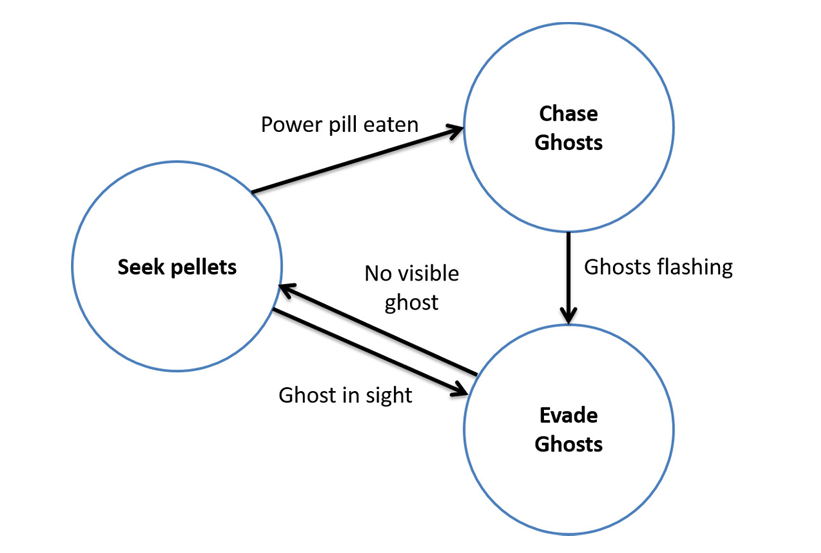
\includegraphics[width = 0.7\textwidth]{Imagenes/FMS_MsPac-man.png}
	\caption{Comportamiento jugador Pac-Man, extraído del libro de Yannakakis y Togelius (2018)}
	\label{fig:Comportamiento jugador Pac-Man}
\end{figure}

Un punto en contra de las FSMs es que son muy inflexibles y estáticas, de manera que las posibilidades de escalado de la lógica son limitadas. También son algo predecibles una vez el jugador ha estudiado los estados y transiciones de una entidad, este punto negativo puede paliarse implementado probabilidades o reglas que no estén tan claras a la hora de hacer las transiciones.

\section{Actuators}
Hablar de los actuators
\subsection{Movement}
Movement contenido a ver si sale guay
\subsubsection{AAAA}
aaaaa
\subsection{Spawner}
Spawner
\section{Sensors and emitters}
Contenido
\subsection{Sensors}
mas contenido
\subsection{Emitters}
muchisimo mas
